%
% T�TULO DEL CAP�TULO
%
\chapter{Technological Foundations
	\label{chapter_2}
}

In this chapter, some Computer Vision concepts are introduced. Paying special attention to our case study that is stereo correspondence. We first introduce what is computer vision and delve into our case study, second we explain the chosen Stereo Matching algorithm and third describe what GPGPU is and its applications in our area of interest. Only a brief description of these concepts is presented, to get more familiarized with Computer Vision the books \cite{computervision} and \cite{computervisionmodern} are recommended. For stereo correspondence techniques, the book chapter \cite{correspondence} is an essential source.

\begin{figure}[h]
	\centering
	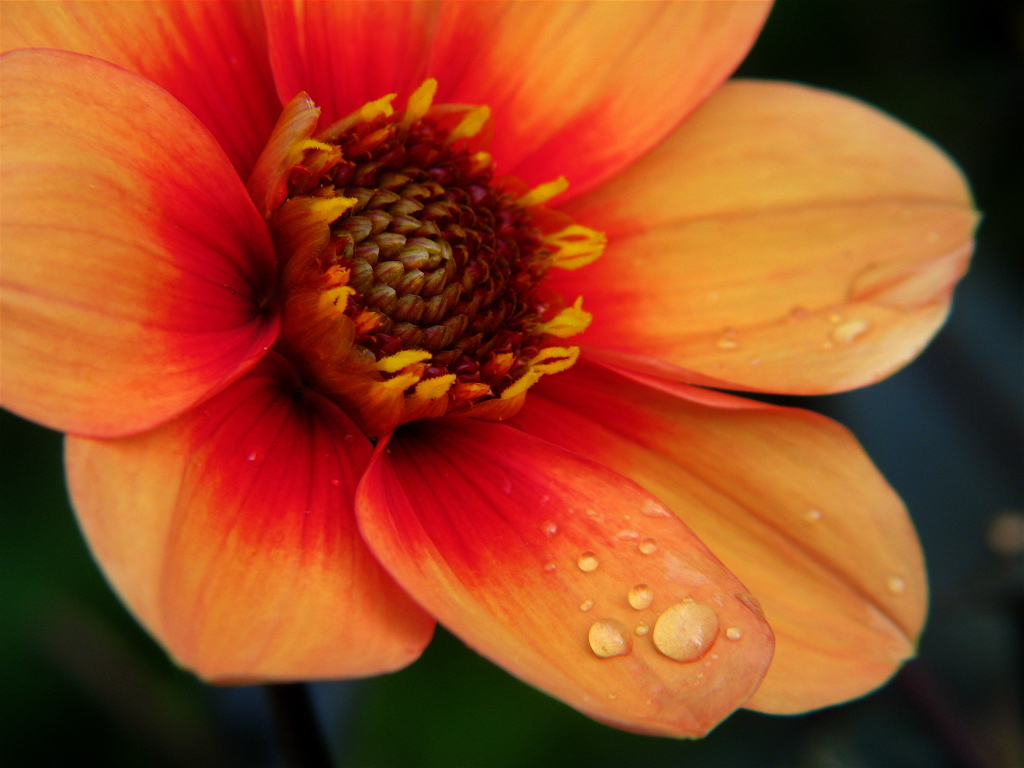
\includegraphics[scale=0.3]{figures/flower.jpg}
	\caption[Background segmentation]{
		The human visual system has no issue interpreting the subtle changes in translucency and shading in this photograph and segmenting the object from its background.
	}
	\label{flower}
\end{figure}

\section{Computer Vision}

As humans, we perceive the tridimensional structure of the world around us with apparent ease. Think of how vivid the tridimensional perception is when one looks at a vase of flowers sitting on the table. You can tell the shape and translucency of each petal through the subtle patterns of light and shading that play across its surface. One can easily segment
each flower from the background of the scene (see \autoref{flower}).

Looking at a framed group portrait, you can effortlessly for example count all of the people and even guess their emotions from their facial appearance. Perceptual psychologists have spent decades trying to understand how the visual system works and, even though they can find optical illusions to tease apart some of its principles (see \autoref{optical_illusion}), a solution to the complete puzzle remains elusive.

\begin{figure}[h]
	\centering
	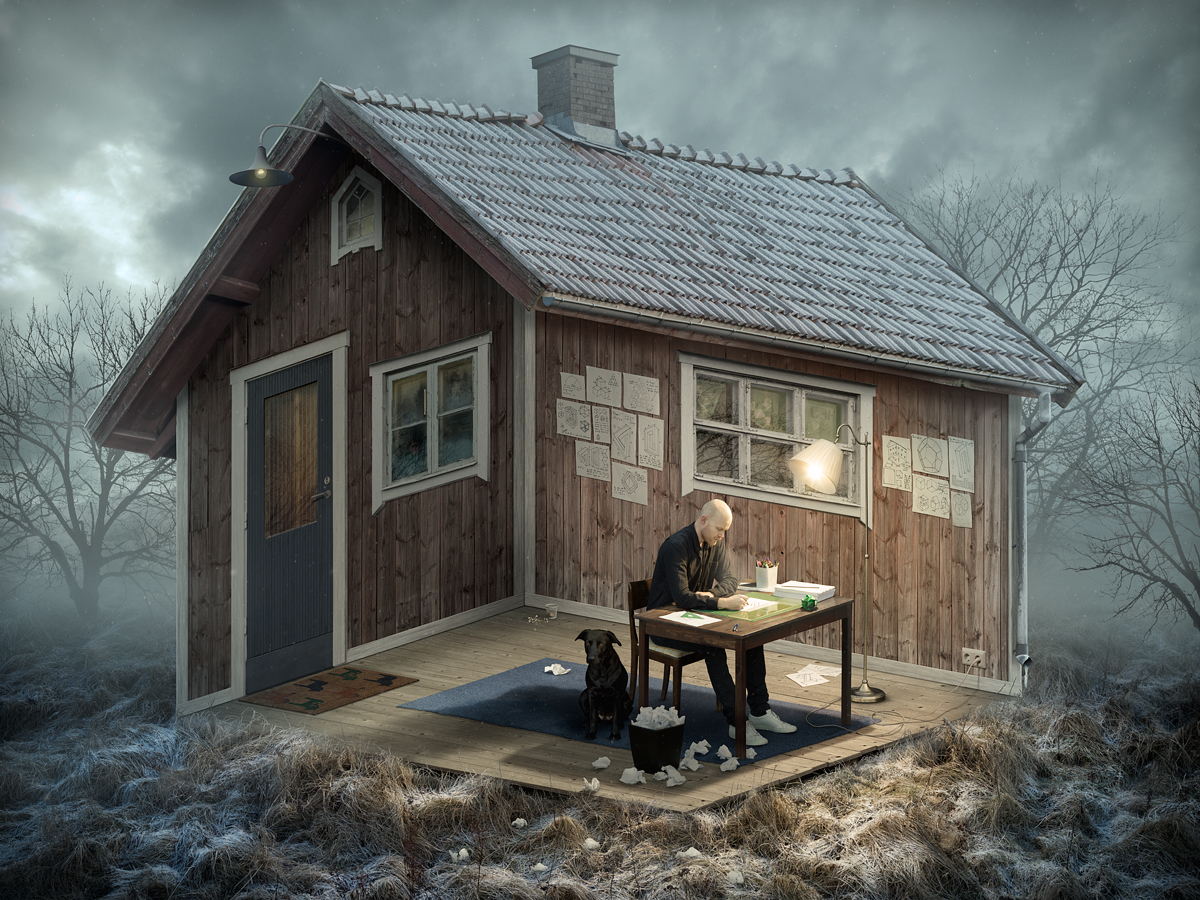
\includegraphics[scale=0.3]{figures/optical_illusion.jpg}
	\caption[Optical illusion]{
		 This work by Eric Johansson is composed of optical illusions that use highly creative pieces that render manipulations of perspective to make the viewer see a perplexed set of images. 
	}
	\label{optical_illusion}
\end{figure}

In areas, such as rendering a still scene composed of everyday objects or animating extinct creatures such as dinosaurs, the illusion of reality is almost perfect. In computer vision, we are trying to do the opposite, i.e., to describe the world that we see in one or a sequence of images and to reconstruct its properties, such as shape, illumination, and color distributions. It is incredible that humans and animals do this so effortlessly, while computer vision algorithms are so error prone.

Applications range from tasks such as industrial machine vision systems which, say, inspect bottles speeding by on a production line, to research into artificial intelligence and computers or robots that can comprehend the world around them. In many computer vision applications, the computers are preprogrammed to solve a certain task, but methods based on learning are now becoming more common. Examples of applications of computer vision include systems for:

\begin{itemize}
\item Process control.
\item Navigation.
\item Event detection. 
\item Information organization.
\item Object or environment modeling.
\item Interaction.
\item Automatic inspection.
\item Etc.
\end{itemize}

Each of the application areas described above employ a range of computer vision tasks; more or less well-defined measurement problems or processing workloads, which can be solved using a variety of methods. Some examples of typical computer vision tasks are presented below:

\begin{itemize}
\item \textbf{Recognition:} the classical problem in computer vision, image processing, and machine vision is that of determining whether or not the image data contains some specific object, feature, or activity.
\item \textbf{Motion analysis:} several tasks relate to motion estimation where an image sequence is processed to produce an estimate of the velocity either at each points in the image or in the 3D scene, or even of the camera that produces the images.
\item \textbf{Scene reconstruction:} Given one or (typically) more images of a scene, or a video, scene reconstruction aims at computing a 3D model of the scene.
\item \textbf{Image restoration:} The aim of image restoration is the removal of noise (sensor noise, motion blur, etc.) from images.
\end{itemize}

\begin{figure}
  \centering
  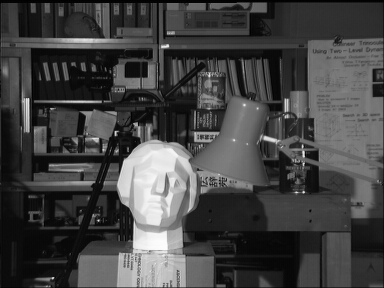
\includegraphics[width=0.475\textwidth]{figures/tsukuba_l.png} \quad
  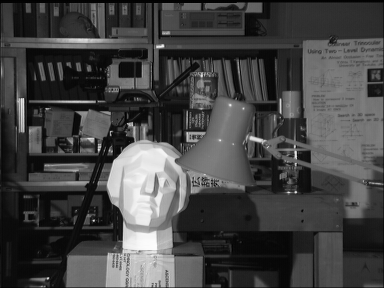
\includegraphics[width=0.475\textwidth]{figures/tsukuba_r.png}
  \caption{Example of stereoscopic images employed in scene reconstruction.}\label{tsukuba_ims}
\end{figure}

Our main interest in this project is \emph{scene reconstruction} from one or more pairs of images (see \autoref{tsukuba_ims}), specifically with stills obtained using stereo vision techniques. This images can be processed to obtain a depth estimation of the scene, once it is known, we have a 3D model of said scene.  

\subsection{Stereo Vision}

Computer stereo vision is the extraction of 3D information from digital images, such as obtained by a CCD camera. By comparing information about a scene from two vantage points, 3D information can be extracted by examination of the relative positions of objects in the two panels. This is similar to the biological process Stereopsis.

\subsection{Stereo Correspondence}

SC

\subsection{Block Matching}

Block Matching

\section{GPGPU}

General-purpose Computing on Graphics Processing Units

\subsection{Architecture}

\subsection{OpenCL}

\subsection{CUDA}